% Chapter 5

\chapter{Conclusions and Future Work} % Main chapter title

\label{Chapter6} % For referencing the chapter elsewhere, use \ref{Chapter5} 

%----------------------------------------------------------------------------------------


%----------------------------------------------------------------------------------------

\section{Conclusions}
We conclude with the present work that TEP problems are suitable for a quantum annealer by providing a formulation for a small network with some simplifications. We test this formulation with D-Wave solvers and it outputs the expected result.\\\\
Lastly, due to the size of TEP problems, the current maturity of quantum computers and the fact that some variables of TEP problems are real, we proposed an hybrid quantum-classical approach based on an iterative method, Benders' decomposition. This open new possibilities to explore TEP problems by combining classical solvers -- that tackle the real and integer parts -- and quantum solvers -- that solve the binary problem -- taking advantage of the key features of each solver.
\section{Future Work}
This master thesis has presented an iterative approach to solve TEP problems, but the data we have used is synthetic. There are different sources of energy models but depending on the source we have to load the data in different ways. We will use the PyPSA python package\,\cite{PyPSA-Eur:PyPSA-Eur} for that task.\\\\
Dealing with real data implies not only dealing with real numbers -- that can be rounded to integers -- but also with a large number of variables which increase the complexity of the problem. These points do not change the implementation, but if we plan to add new components such as storages -- which implies taking into account a multi-snapshot dependence -- the linear equations that describe our problem are going to change. PyPSA can simplify the linear model for any number of targets considered in the original problem and to plot of the associated network for a given number of nodes $N$, Figure\,\ref{fig:GeneralNetworks}.This enables us to read these linear equations and include it into our Benders' decomposition scheme. For this task we plan to use QUARK\,\cite{dlrsc2023quark}, a reformulation kernel that allows us to send the algorithm to different quantum machines.
\begin{figure}[H]
\centering
\begin{subfigure}[c]{0.5\linewidth}
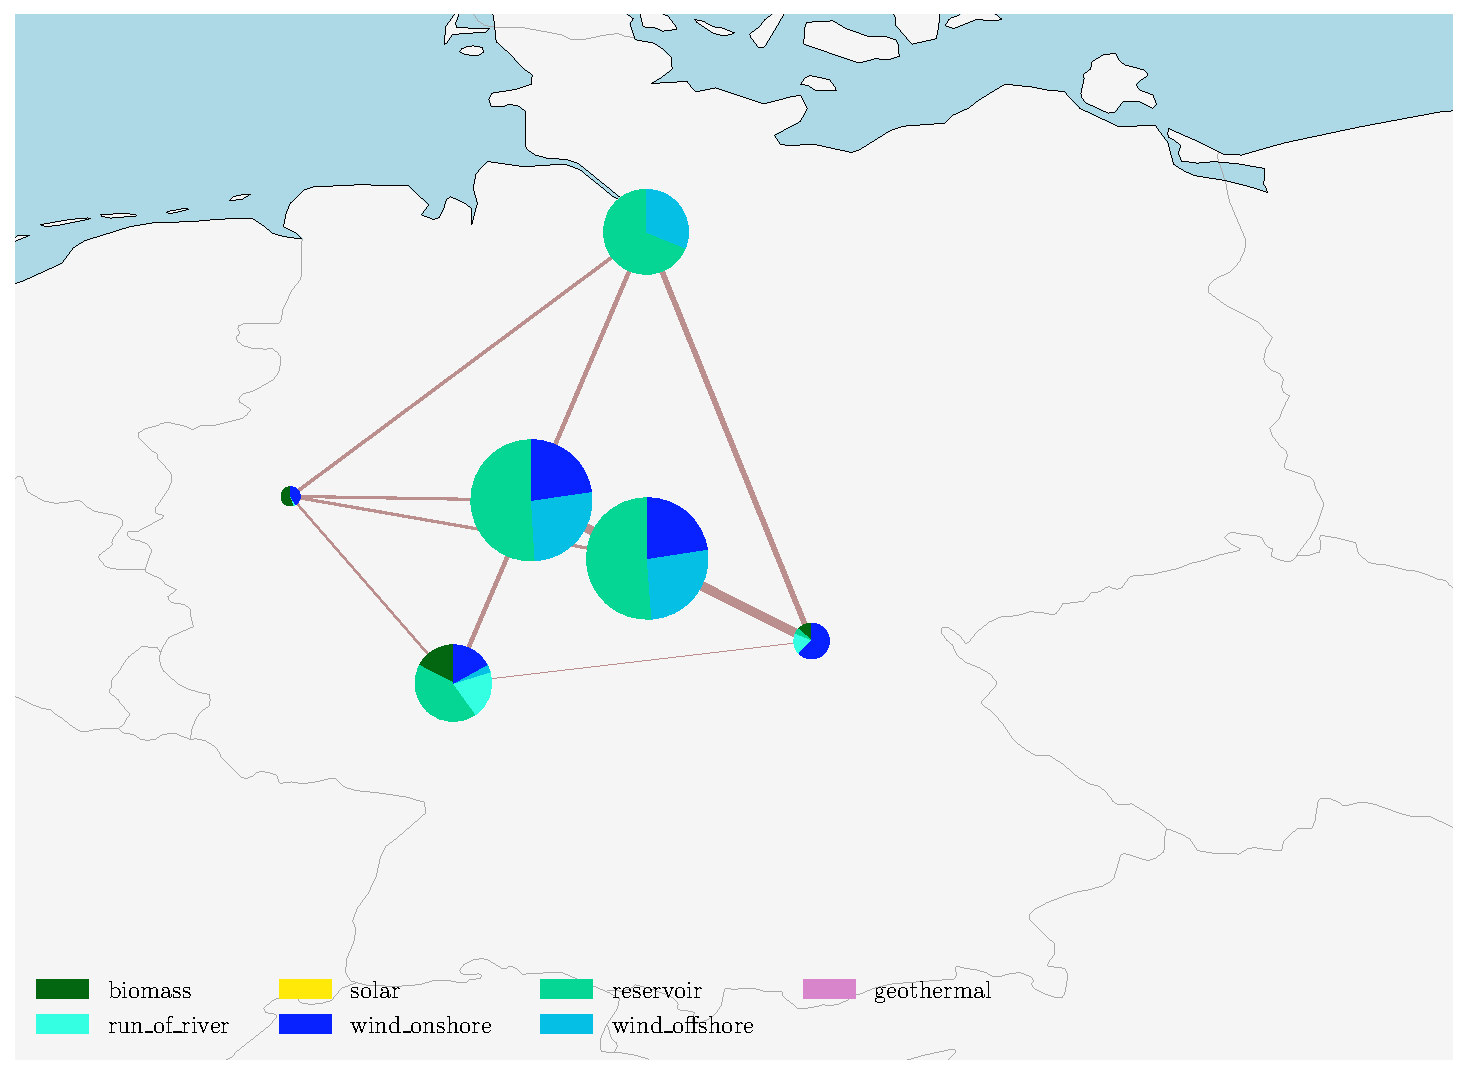
\includegraphics[width=\linewidth]{Figures/eGo100_No4.pdf} 
\caption{$N=6$.}
\label{fig:3a}
\end{subfigure}\hfill    
\begin{subfigure}[c]{0.5\linewidth}
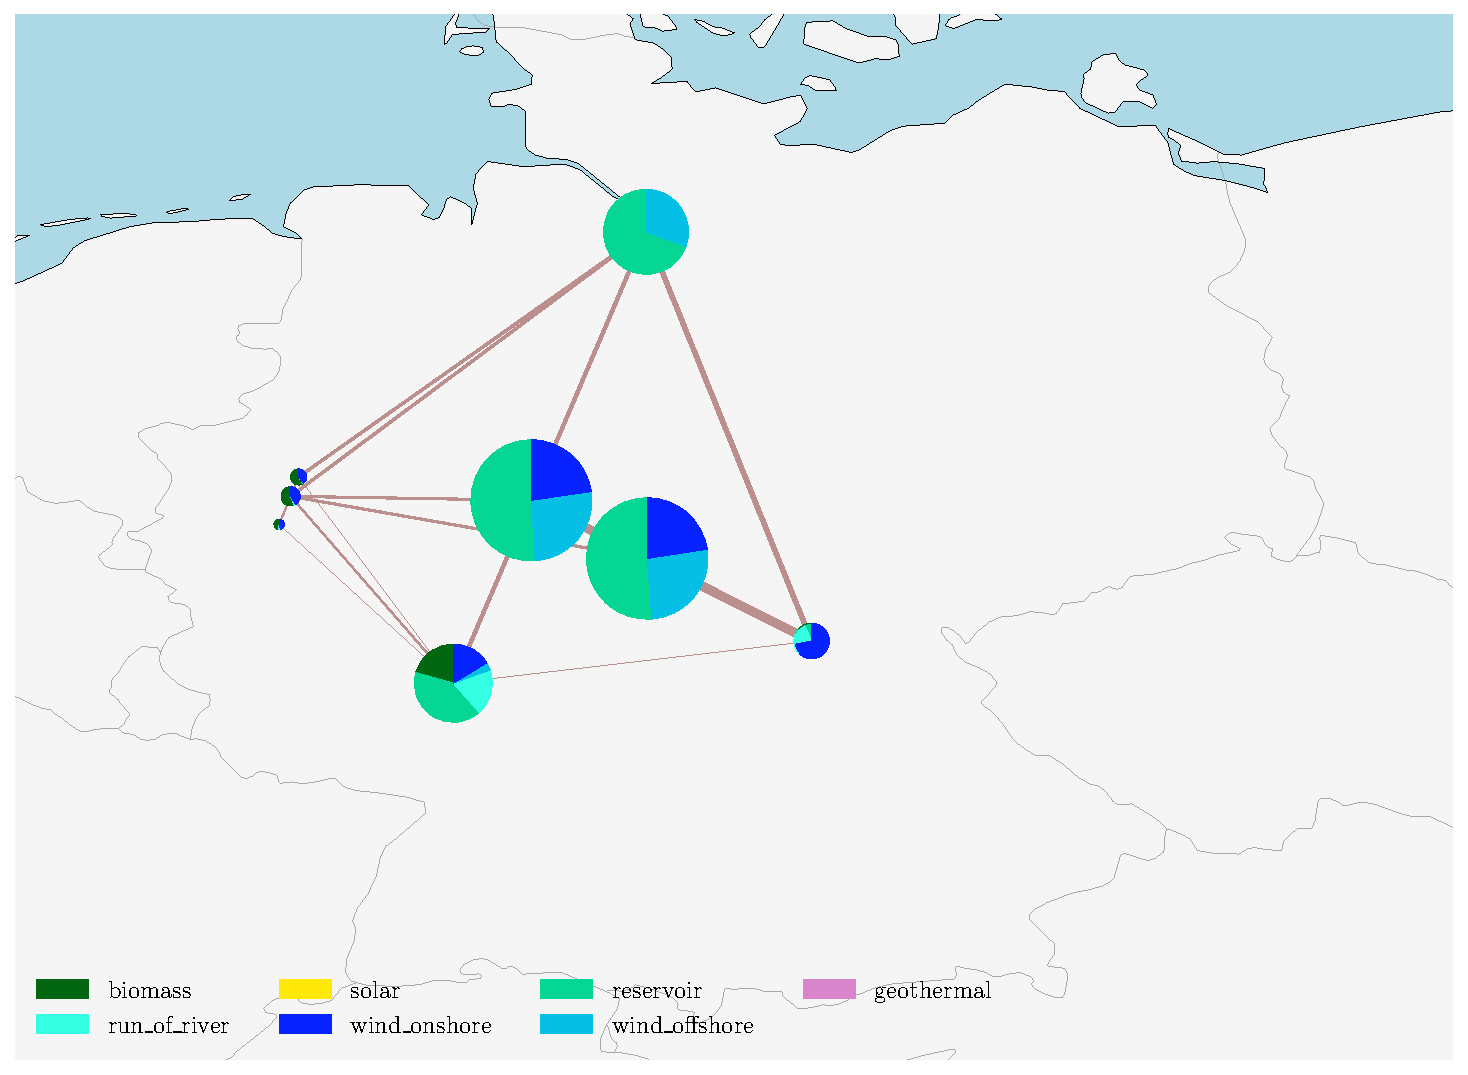
\includegraphics[width=\linewidth]{Figures/eGo100_No5.pdf}
\caption{$N=8$.}
\label{fig:3b}
\end{subfigure}
%add desired spacing between images, e. g. ~, \quad, \qquad, \hfill etc. 
%(or a blank line to force the subfigure onto a new line)
\begin{subfigure}[c]{0.5\linewidth}
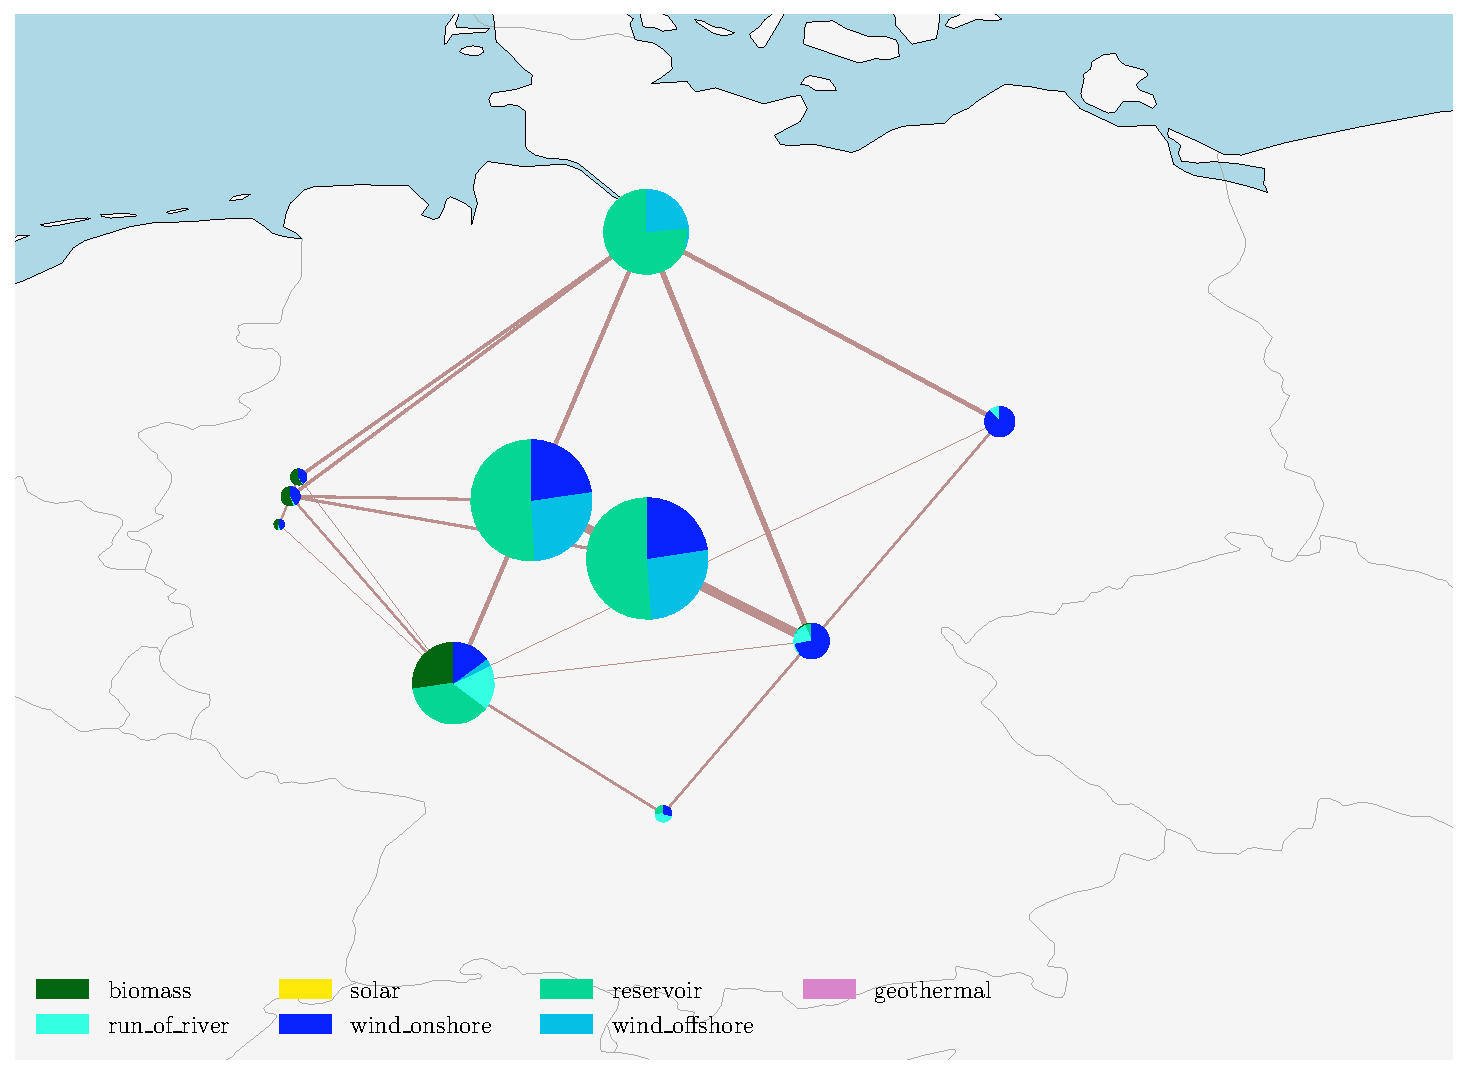
\includegraphics[width=\linewidth]{Figures/eGo100_No6.pdf}
\caption{$N=10$.}
\label{fig:3c}
\end{subfigure}\hfill    
\begin{subfigure}[c]{0.5\linewidth}
\includegraphics[width=\linewidth]{Figures/eGo100_No7.pdf}
\caption{$N=12$.}
\label{fig:3d}
\end{subfigure}
    
\caption{Germany network generated with PyPSA for $N$ cluster from eGo100 data\,\cite{Mueller2018}.}
\label{fig:GeneralNetworks}
\end{figure}
Last, we could compare our hybrid quantum-classical algorithm with the ones provided by the quantum solvers. We think that a specific hybrid quantum-classical approach should provide a better solution in term of computational time and optimal value than the general hybrid solvers from D-Wave. Furthermore, we should be able to determine the exact usage of quantum solver we employing in the problem, which is not possible with solvers such as D-Wave.